\documentclass{standalone}
\usepackage{tikz}
\usetikzlibrary{arrows.meta}

\begin{document}

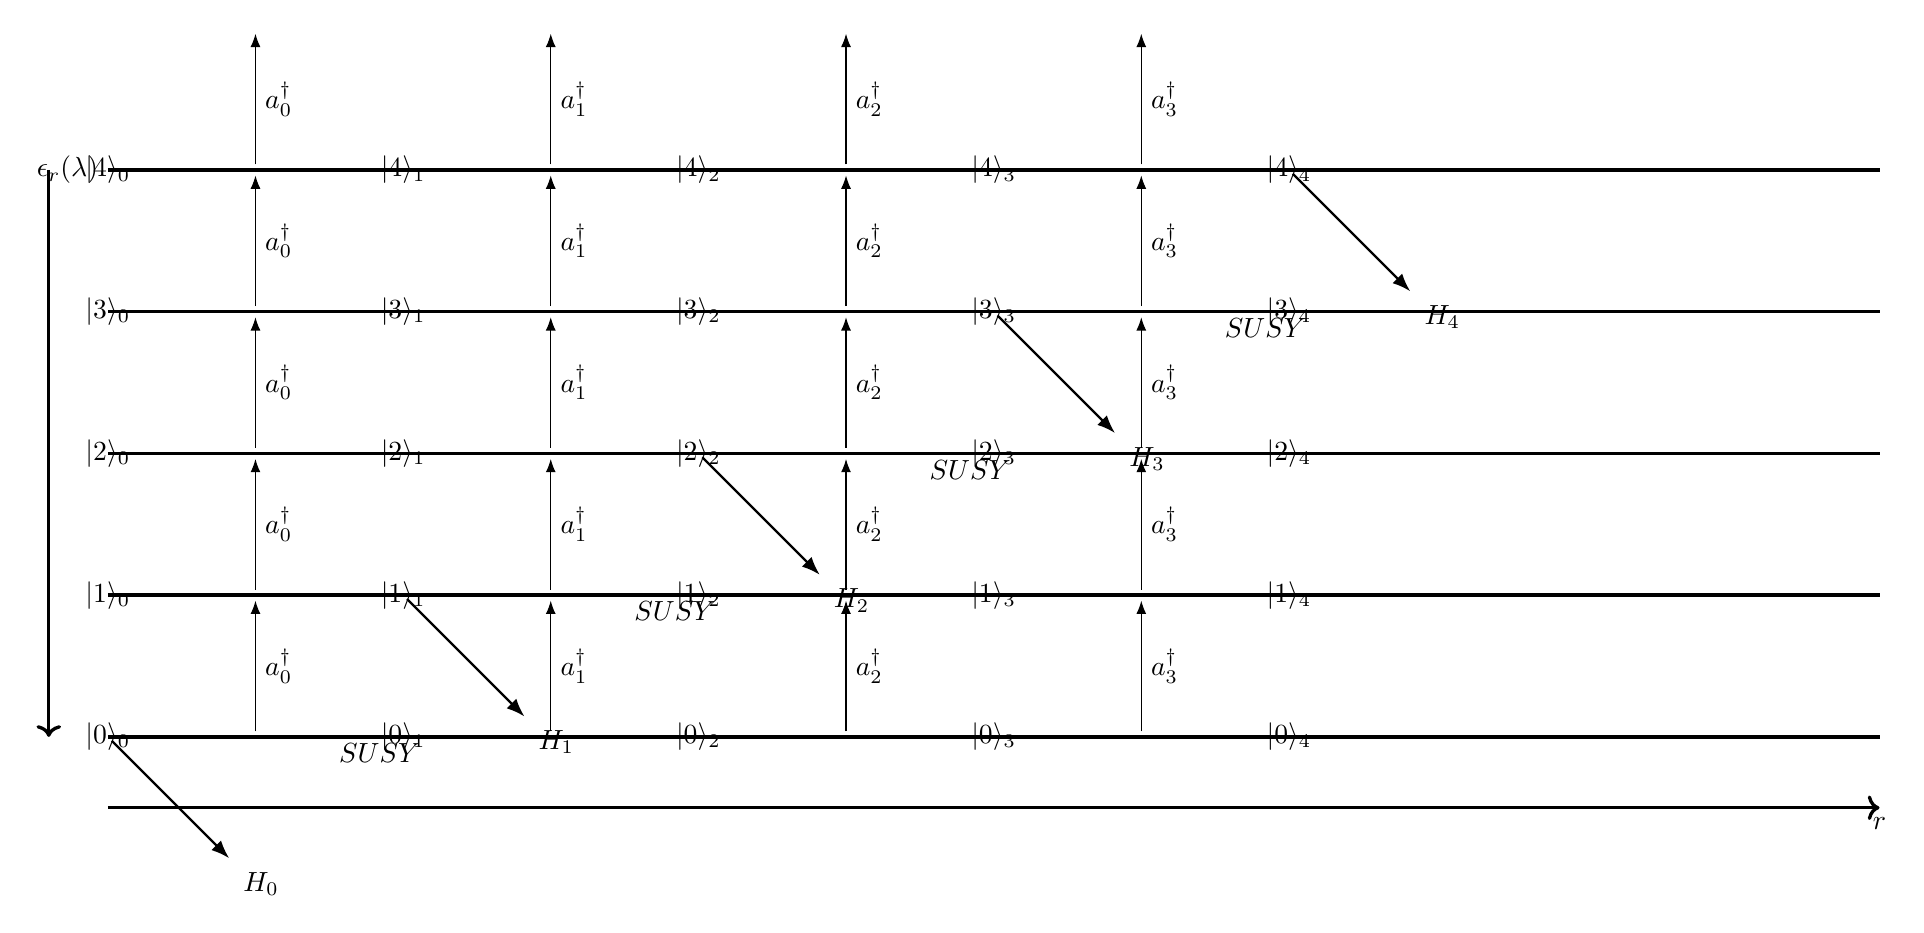
\begin{tikzpicture}[scale=1.5]

% Define some constants for positioning
\def\xshift{2.5} % Horizontal spacing between lines
\def\yshift{-1.2} % Vertical spacing between energy levels

% Draw horizontal lines representing energy levels
\foreach \n in {0,...,4} {
    \draw[very thick] (0,\n*\yshift) -- (\xshift*6,\n*\yshift);
}

% Place the states and arrows
\foreach \n [evaluate=\n as \level using int(4-\n)] in {0,...,4} {
    \foreach \m in {0,...,4} {
        \node at (\m*\xshift,\n*\yshift) {$|\level\rangle_{\m}$};
        \ifnum\m<4
            \draw[-Latex, shorten >=2pt, shorten <=2pt] 
                (\m*\xshift+0.5*\xshift,\n*\yshift) -- ++(0,-\yshift)
                node[midway, right] {$a^{\dagger}_{\m}$};
        \fi
    }
}

% Add vertical axis label
\node[left] at (0,0) {$\epsilon_r(\lambda)$};
\draw[->, very thick] (-0.5,0) -- (-0.5,4*\yshift);

% Add horizontal axis label
\node[below] at (\xshift*6,\yshift*4.5) {$r$};
\draw[->, very thick] (0,\yshift*4.5) -- (\xshift*6,\yshift*4.5);

% Add SUSY connections
\draw[thick, -Latex, shorten >=2pt, shorten <=2pt] 
    (0,\yshift*4) -- ++(-45:1.5) node[below right] {$H_0$};
\draw[thick, -Latex, shorten >=2pt, shorten <=2pt] 
    (\xshift,\yshift*3) -- ++(-45:1.5) node[below right] {$H_1$};
\draw[thick, -Latex, shorten >=2pt, shorten <=2pt] 
    (\xshift*2,\yshift*2) -- ++(-45:1.5) node[below right] {$H_2$};
\draw[thick, -Latex, shorten >=2pt, shorten <=2pt] 
    (\xshift*3,\yshift*1) -- ++(-45:1.5) node[below right] {$H_3$};
\draw[thick, -Latex, shorten >=2pt, shorten <=2pt] 
    (\xshift*4,\yshift*0) -- ++(-45:1.5) node[below right] {$H_4$};

% Add "SUSY" labels
\node[above right] at (\xshift*0.75,\yshift*4.25) {$SUSY$};
\node[above right] at (\xshift*1.75,\yshift*3.25) {$SUSY$};
\node[above right] at (\xshift*2.75,\yshift*2.25) {$SUSY$};
\node[above right] at (\xshift*3.75,\yshift*1.25) {$SUSY$};

\end{tikzpicture}

\end{document}